\documentclass[conference,a4paper]{IEEEtran}
\IEEEoverridecommandlockouts
\usepackage[T1]{fontenc}
\usepackage{mathptmx}
\usepackage{cite}
\usepackage{amsmath,amssymb,amsfonts}
\usepackage{graphicx}
\usepackage{textcomp}
\usepackage{xcolor}
\usepackage{url}
\usepackage{array}
\def\BibTeX{{\rm B\kern-.05em{\sc i\kern-.025em b}\kern-.08em T\kern-.1em\lower.7ex\hbox{E}\kern-.125em X}}
\begin{document}

\title{Predicting 30-Day Hospital Readmission in Indian Hospitals: Machine Learning and Deep Learning Models with a Study-Design Audit}

\author{\begin{tabular}{@{}c@{}}
\begin{minipage}[t]{0.32\textwidth}\centering
{\normalsize\textit{1\textsuperscript{st} Premkumar Duraisamy}}\\[1pt]
{\footnotesize Department of Computer Science\\and Engineering\\
\textit{KPR Institute of Engineering and Technology}\\
Coimbatore, India\\
technicalprem@gmail.com}
\end{minipage}\hfill\begin{minipage}[t]{0.32\textwidth}\centering
{\normalsize\textit{2\textsuperscript{nd} Ragav K}}\\[1pt]
{\footnotesize Department of Computer Science\\and Engineering\\
\textit{KPR Institute of Engineering and Technology}\\
Coimbatore, India\\
iamragav2k7@gmail.com}
\end{minipage}\hfill\begin{minipage}[t]{0.32\textwidth}\centering
{\normalsize\textit{3\textsuperscript{rd} Narendran R N}}\\[1pt]
{\footnotesize Department of Computer Science\\and Engineering\\
\textit{KPR Institute of Engineering and Technology}\\
Coimbatore, India\\
narenravi1511@gmail.com}
\end{minipage}\\
\noalign{\vskip 12pt}
\begin{minipage}[t]{0.32\textwidth}\centering
{\normalsize\textit{4\textsuperscript{th} Nilavan K}}\\[1pt]
{\footnotesize Department of Computer Science\\and Engineering\\
\textit{KPR Institute of Engineering and Technology}\\
Coimbatore, India\\
knilavan06@gmail.com}
\end{minipage}\hfill\begin{minipage}[t]{0.32\textwidth}\centering
{\normalsize\textit{5\textsuperscript{th} Pagalavan K}}\\[1pt]
{\footnotesize Department of Computer Science\\and Engineering\\
\textit{KPR Institute of Engineering and Technology}\\
Coimbatore, India\\
kpagalavan06@gmail.com}
\end{minipage}\hfill\begin{minipage}[t]{0.32\textwidth}\centering
{\normalsize\textit{6\textsuperscript{th} Sanjay M S}}\\[1pt]
{\footnotesize Department of Computer Science\\and Engineering\\
\textit{KPR Institute of Engineering and Technology}\\
Coimbatore, India\\
24cs182@kpriet.ac.in}
\end{minipage}
\end{tabular}}

\maketitle

\begin{abstract}
Hospital readmission within 30 days of discharge is a common marker of care quality, and models that flag high-risk patients could help plan follow-up. This work tests how well routine admission records predict 30-day readmission in a public India hospital dataset of five linked tables with 120,000 admissions from 33 hospitals. Records were checked, merged, imputed, one-hot encoded and split by patient. A prior-only baseline, logistic regression, random forest, XGBoost and a multilayer perceptron (MLP) were trained with class weighting, and thresholds were set on validation data. After excluding in-hospital deaths, 112,587 admissions remained, of which 12.6\% were readmitted. On the test set the four models reached ROC-AUC values of 0.748 to 0.756, with overlapping 95\% intervals, against 0.500 for the baseline. Logistic Regression scored highest (0.756) and MLP had the highest recall (0.503). A design audit showed that keeping in-hospital deaths raised ROC-AUC by about 0.020, whereas random instead of patient-grouped splitting changed it by less than 0.001. Careful cohort definition therefore matters more than model choice here.
\end{abstract}

\vspace{2pt}
\noindent\textbf{\textit{Keywords---}}\textit{hospital readmission, machine learning, deep learning, class imbalance, study design}

\section{Introduction}
Readmission to hospital soon after discharge is costly for patients and hospitals, and the 30-day readmission rate is widely used as a quality indicator. A systematic review found that most published risk models performed poorly, with c-statistics from 0.55 to 0.83 depending on the data used and the timing of prediction \cite{kansagara}. Better risk ranking would let hospitals direct follow-up to the patients who need it most.

Machine learning is now common in this area. Studies have applied boosting and neural networks to hospital records and reported gains over older scores such as LACE \cite{davis,silva}. A recent umbrella review describes ensemble and neural models as frequent top performers \cite{alrazeeni}, yet a meta-analysis of heart-failure studies pooled an AUC of only 0.733 for the best readmission model \cite{hajishah}. A systematic review also found no evidence that machine learning beats logistic regression when studies are free of validation bias \cite{christodoulou}. Results therefore depend on the data and on how models are compared.

Indian evidence is limited. Published work includes a 352-record diabetes clinic study \cite{mishra} and an audit of older adults in one geriatric unit that reported a 5.18\% readmission rate but built no prediction model \cite{samuel}. Readmission is also a rare event, so accuracy alone is misleading and precision--recall measures are needed \cite{saito2015pr}. Deep networks are not always better than trees on tabular data \cite{grinsztajn2022tree}.

This work uses the public India Hospital Readmission Dataset (2015--2024) \cite{kaggle}, which links admissions, patients, diagnoses, billing and hospitals. In this work, the main steps include checking and merging five tables, excluding in-hospital deaths, splitting by patient, and training a prior-only baseline and four models with class weighting. The experimental results are used to compare the models and to measure how two design choices change reported performance. The contributions are: (i) a leakage-aware pipeline for linked hospital tables, (ii) a like-for-like comparison of three machine learning models and one deep learning model, with confidence intervals and a baseline, and (iii) a design audit of keeping in-hospital deaths and of using a random split. Reporting was guided by the TRIPOD+AI recommendations \cite{collins2024}, and the items that this work does not cover are stated in Section~V.

\section{Literature Review}
Table~I lists eight recent studies. Davis et al.\ combined learned and hand-made features in a gradient boosting model and raised AUC from 0.66 (LACE) to 0.83 on Alberta administrative data \cite{davis}. Silva et al.\ found XGBoost best for children \cite{silva}. Gao et al.\ showed that a regression tree extracted from a neural network can keep accuracy while staying readable \cite{gao}. Loutati et al.\ added a text-based score to structured data for elderly patients \cite{loutati}. In India, Mishra et al.\ reported XGBoost as best on a very small clinic dataset \cite{mishra}, and Samuel et al.\ measured readmission in older adults without modelling it \cite{samuel}. Hajishah et al.\ pooled 64 heart-failure studies and noted a high risk of bias \cite{hajishah}, and an umbrella review of emergency patients found ensemble and neural models frequently strong \cite{alrazeeni}.

Three gaps remain. Few studies compare models on large multi-hospital Indian data, few report uncertainty around the model ranking, and the effect of cohort definition on reported performance is rarely quantified. This work addresses all three.

\begin{table*}[!t]
\caption{Comparison of Related Work}
\label{tab:lit}
\centering\footnotesize\renewcommand{\arraystretch}{1.1}\setlength{\tabcolsep}{3pt}
\begin{tabular}{|c|c|>{\raggedright\arraybackslash}p{1.5in}|>{\raggedright\arraybackslash}p{1.35in}|>{\raggedright\arraybackslash}p{1.6in}|>{\raggedright\arraybackslash}p{1.4in}|}
\hline
\textbf{Year} & \textbf{Ref.} & \textbf{Dataset/Application} & \textbf{Method} & \textbf{Main Finding} & \textbf{Limitation} \\\hline
2026 & \cite{alrazeeni} & Emergency patients (umbrella review) & AI, ML and DL models from reviews & Ensemble and neural models often strong; EHR data helps & Review only; no new model comparison \\
2025 & \cite{mishra} & 352 records, diabetes clinic, Varanasi, India & LR, DT, RF, XGBoost & XGBoost F1 0.85; RF AUC-ROC 0.94 & Very small, single clinic \\
2025 & \cite{hajishah} & 64 heart-failure studies, 943,941 patients & Meta-analysis of ML models & SVM best for readmission (pooled AUC 0.733) & High risk of bias; retrospective data \\
2024 & \cite{loutati} & 19,569 admissions, age $\geq$75, Israel & Multimodal ML with text score & AUROC 0.87--0.93 & Single centre; elderly only \\
2023 & \cite{silva} & 9,080 paediatric patients, tertiary hospital & CART, RF, GBM, XGBoost, DT, LR & XGBoost best (AUC 0.814) & Single hospital; children only \\
2023 & \cite{gao} & Large teaching hospital, Asia & Neural net + extracted regression tree & Similar AUC and AUPRC to black box; readable & Single hospital \\
2022 & \cite{davis} & 428,669 patients, Alberta, Canada & GBM with learned + manual features & AUC 0.83 vs 0.66 for LACE & Administrative data; 5.8\% readmit rate \\
2022 & \cite{samuel} & 2,698 older adults, Vellore, India & Retrospective chart audit (no ML) & 30-day readmission 5.18\%; 41.4\% potentially avoidable & Older adults, one hospital; no prediction model \\
\hline
\end{tabular}
\end{table*}

\section{Proposed System}
As shown in Fig.~\ref{fig:flow}, the work follows a sequence of data checking, preprocessing, model training and evaluation steps. Fig.~\ref{fig:arch} shows the best-performing model.

\begin{figure}[!t]
\centering
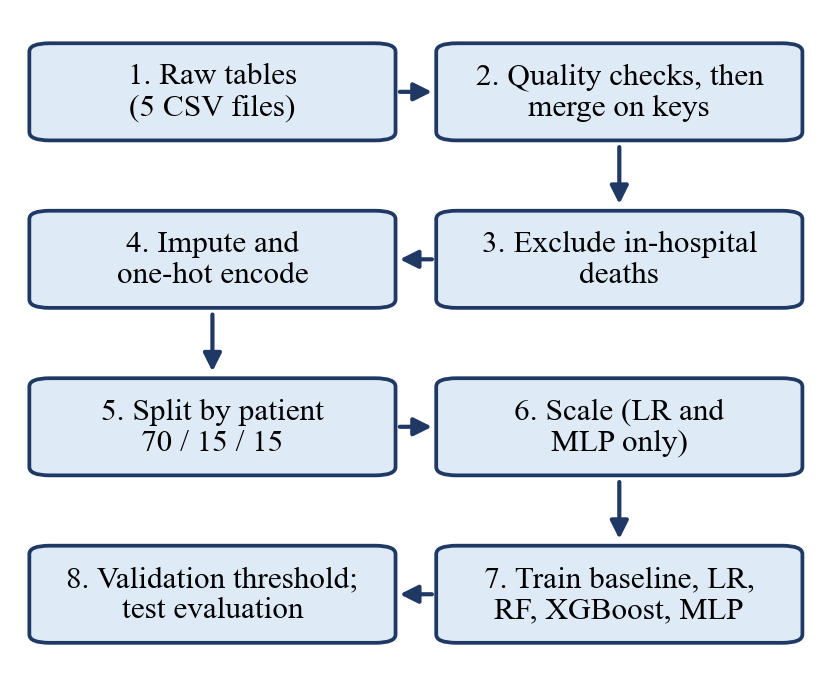
\includegraphics[width=\columnwidth]{figs/fig1_workflow.png}
\caption{Overall workflow of the proposed work.}
\label{fig:flow}
\end{figure}

\subsection{Data Acquisition}
Five linked tables were used: admissions (120,000 rows), patients (86,400), diagnoses (271,341), billing (120,000) and hospitals (33) \cite{kaggle}. One row of the final table is one admission. The label is the supplied \texttt{readmitted\_30d} field. The process that generated it is not documented, so it was taken as given.

\subsection{Data Preprocessing}
Every table was checked first. No table had missing cells or duplicate rows, all keys were unique, every admission linked to one patient, one hospital, one bill and a rank-1 diagnosis, and no impossible values were found (negative stays, out-of-range ages or laboratory values, inconsistent dates). The string ``None'' in the insurance field (28.6\% of patients) means no insurance and was kept as its own category, not treated as missing. Extreme values were kept as clinically plausible; for example, 4.8\% of stays and 7.6\% of HbA1c values lie outside the 1.5 IQR rule.

Patients who died in hospital cannot be readmitted, and none of the 7,413 such admissions carried a readmission flag, so they were excluded. The 7-day flag was not used as an input because it is part of the outcome. A patient can have several admissions, and 34,978 patients do.

\subsection{Feature Preparation}
The tables were joined on patient, hospital and admission keys, and the rank-1 diagnosis gave the primary diagnosis. Dates gave admission year and month, and billing gave cost per day and out-of-pocket share. Numeric fields were median-imputed, although none were missing. The 9 categorical fields were one-hot encoded, giving 71 input columns. Standard scaling was applied only for logistic regression and the MLP. Length of stay, laboratory values, discharge type and billing are known only near discharge, so the task is discharge-time prediction.

\subsection{Model Training}
The split was grouped by patient to avoid leakage (70\% training, 15\% validation, 15\% test). A prior-only baseline that always predicts the training prevalence was added as a floor. Logistic regression is the linear baseline, random forest averages many decision trees, and XGBoost \cite{chen2016xgboost} builds trees in sequence, each correcting the earlier ones. The MLP is the deep learning model. Class imbalance was handled with class weights, so no synthetic samples were created.

\subsection{Model Evaluation}
For each model, the decision threshold was chosen on the validation set to maximise F1 and then fixed for the test set. Accuracy, precision, recall, F1, ROC-AUC, PR-AUC and the Brier score were computed, with 95\% bootstrap intervals for ROC-AUC (300 resamples). A robustness check trained on admissions before 2024 and tested on 2024.

\subsection{Prediction and Best Model}
The model outputs a readmission probability for each admission, which is turned into a high-risk flag by the validation threshold. By test ROC-AUC, Logistic Regression performed best (Table~III). It is a linear model on 71 scaled inputs whose weighted sum passes through a sigmoid, as shown in Fig.~\ref{fig:arch}, and its coefficients are directly readable.

\begin{figure}[!t]
\centering
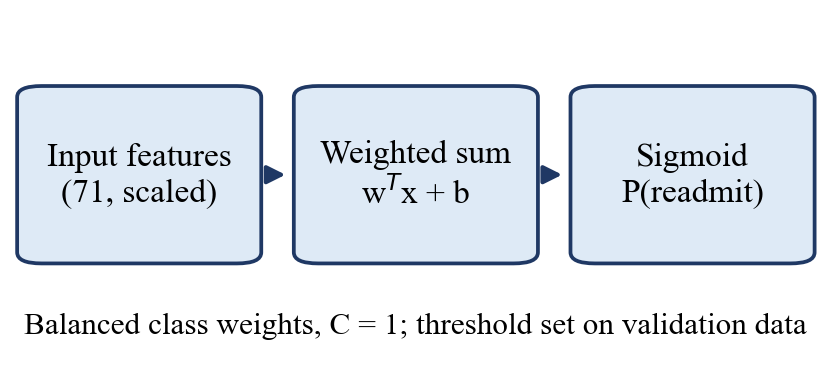
\includegraphics[width=\columnwidth]{figs/fig2_architecture.png}
\caption{Architecture of the best-performing model (Logistic Regression).}
\label{fig:arch}
\end{figure}

\section{Experimental Setup}
All code was written in Python 3.13.15 with scikit-learn 1.6.1, XGBoost 3.4.1 and PyTorch 2.11.0, with a fixed seed (42), and was run on a Google Colab CPU runtime (2 cores). The modelling cohort has 112,587 admissions of 62,923 patients, with 14,210 readmissions (12.6\%) and 71 input columns. The target is \texttt{readmitted\_30d}. The train, validation and test sets hold 78,758, 16,930 and 16,899 admissions, and the test set has 2,153 readmissions (12.7\%). Table~II presents the inputs and the preprocessing steps used in the work.

Logistic regression used $C{=}1$, an L2 penalty, the lbfgs solver, up to 2000 iterations and balanced class weights (1.6 s). The random forest used 300 trees, maximum depth 12, minimum leaf size 20, sqrt features per split and balanced-subsample weights (32.1 s). XGBoost used depth 5, learning rate 0.05, up to 400 trees with early stopping after 30 rounds (stopped at 71), row and column sampling of 0.8, and \texttt{scale\_pos\_weight} 6.98 (5.4 s). The MLP had hidden layers of 128, 64, 32 units with ReLU and dropout 0.3, and was trained with Adam (learning rate 0.001), batch size 512, a class-weighted binary cross-entropy loss and early stopping with patience 6; it ran 13 epochs (14.8 s). Hyperparameters were fixed in advance and were not tuned on the test set.

\begin{table}[!t]
\caption{Dataset and Preprocessing Summary}
\label{tab:data}
\centering\footnotesize\renewcommand{\arraystretch}{1.1}\setlength{\tabcolsep}{3pt}
\begin{tabular}{|>{\raggedright\arraybackslash}p{1.25in}|>{\centering\arraybackslash}p{0.65in}|>{\raggedright\arraybackslash}p{1.2in}|}
\hline
\textbf{Feature Category} & \textbf{Number} & \textbf{Processing Method} \\\hline
Numeric (stay, labs, age, cost, hospital, time) & 21 & Median imputation; scaled for LR and MLP \\\hline
Categorical (admission, ward, discharge, sex, state, insurance, tier, cost type, diagnosis) & 9 $\rightarrow$ 50 columns & One-hot encoding \\\hline
Target & 1 & 30-day readmission (12.6\% positive) \\\hline
Removed inputs & 3 groups & IDs and dates; 7-day flag; 7,413 in-hospital deaths \\\hline
Split (by patient) & 78,758 / 16,930 / 16,899 & Train / validation / test \\\hline
\end{tabular}
\end{table}

\section{Results and Discussion}
Table~III compares the models on the test set, and Fig.~\ref{fig:bars} shows the same scores. The prior-only baseline reached 0.873 accuracy by predicting no readmissions, with zero recall and ROC-AUC of 0.500, which shows why accuracy alone is misleading. The four learned models reached ROC-AUC between 0.748 and 0.756. Logistic Regression had the highest ROC-AUC (0.756, 95\% interval 0.743--0.767), PR-AUC (0.372), accuracy, precision and F1 (0.3997 against 0.3967 for MLP), while MLP had the highest recall (0.503). The intervals overlap for all four models, so the gaps are small and should not be read as a real ranking. This agrees with the finding that machine learning shows no clear benefit over logistic regression on clinical prediction tasks \cite{christodoulou} and with evidence that tree models and neural networks perform alike on medium-sized tabular data \cite{grinsztajn2022tree}. A likely reason is that the strong signals, such as stay length, comorbidity and ward, act mostly in a simple additive way.

\begin{table}[!t]
\caption{Performance Comparison of Machine Learning Models}
\label{tab:perf}
\centering\footnotesize\setlength{\tabcolsep}{2.6pt}
\begin{tabular}{|l|c|c|c|c|c|c|c|}
\hline
\textbf{Model} & \textbf{Acc.} & \textbf{Prec.} & \textbf{Rec.} & \textbf{F1} & \textbf{AUC} & \textbf{PR-AUC} & \textbf{Brier} \\\hline
Logistic Reg. & \textbf{0.828} & \textbf{0.360} & 0.449 & \textbf{0.400} & \textbf{0.756} & \textbf{0.372} & 0.201 \\
Random Forest & 0.809 & 0.326 & 0.468 & 0.384 & 0.748 & 0.350 & \textbf{0.176} \\
XGBoost & 0.807 & 0.327 & 0.490 & 0.392 & 0.752 & 0.365 & 0.199 \\
MLP (DL) & 0.805 & 0.327 & \textbf{0.503} & 0.397 & 0.754 & 0.369 & 0.205 \\
\hline
Prior-only & 0.873 & 0.000 & 0.000 & 0.000 & 0.500 & 0.127 & 0.111 \\
\hline
\end{tabular}
\end{table}

\begin{figure}[!t]
\centering
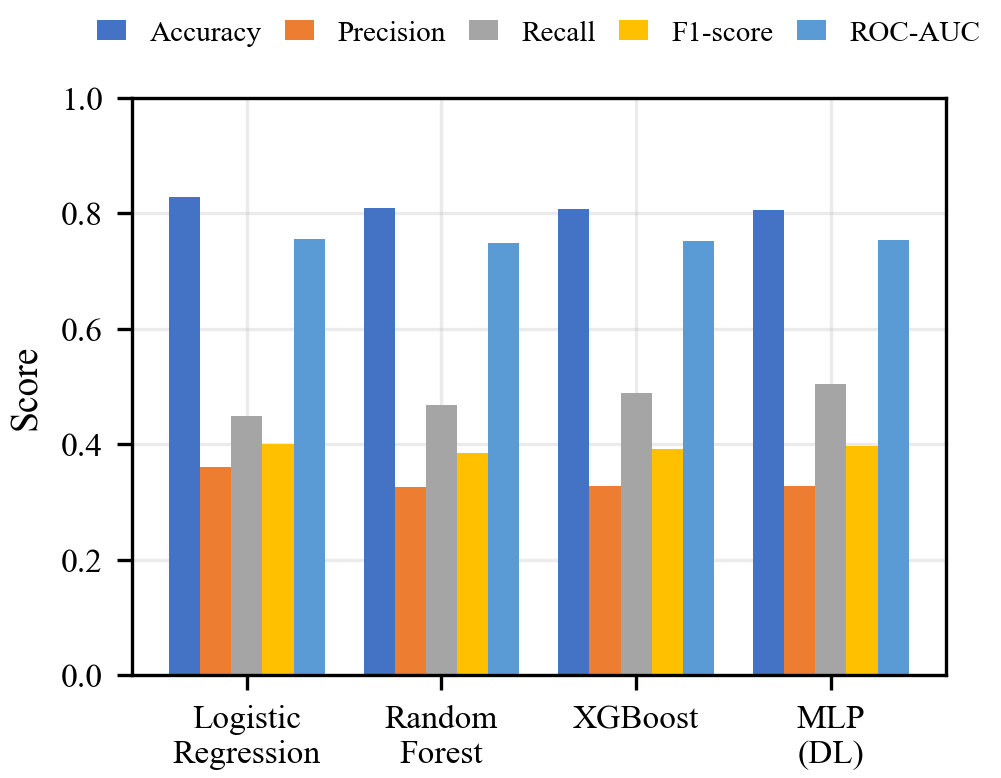
\includegraphics[width=\columnwidth]{figs/fig3_model_comparison.png}
\caption{Accuracy, precision, recall, F1-score and ROC-AUC of the four learned models on the test set.}
\label{fig:bars}
\end{figure}

The confusion matrix in Fig.~\ref{fig:cm} gives the class-wise results. At the chosen threshold, Logistic Regression correctly flagged 967 of 2,153 readmissions (recall 0.449) and missed 1,186, and it raised 1,719 false alarms (specificity 0.883). Among admissions predicted as not readmitted, 91.7\% were correct, but only 36.0\% of flagged admissions were true readmissions. The threshold was tuned for F1, so a hospital that values recall over precision could lower it. The Brier scores of the class-weighted models (0.176--0.205) are worse than that of the prior-only baseline (0.111), so their outputs should be read as rankings, not absolute risks, unless they are recalibrated. As Fig.~\ref{fig:roc} shows, the ROC and precision--recall curves of all four models nearly overlap. Because readmission is rare, the precision--recall view is the more informative one \cite{saito2015pr}, and all curves lie far above the no-skill line (12.7\%).

\begin{figure}[!t]
\centering
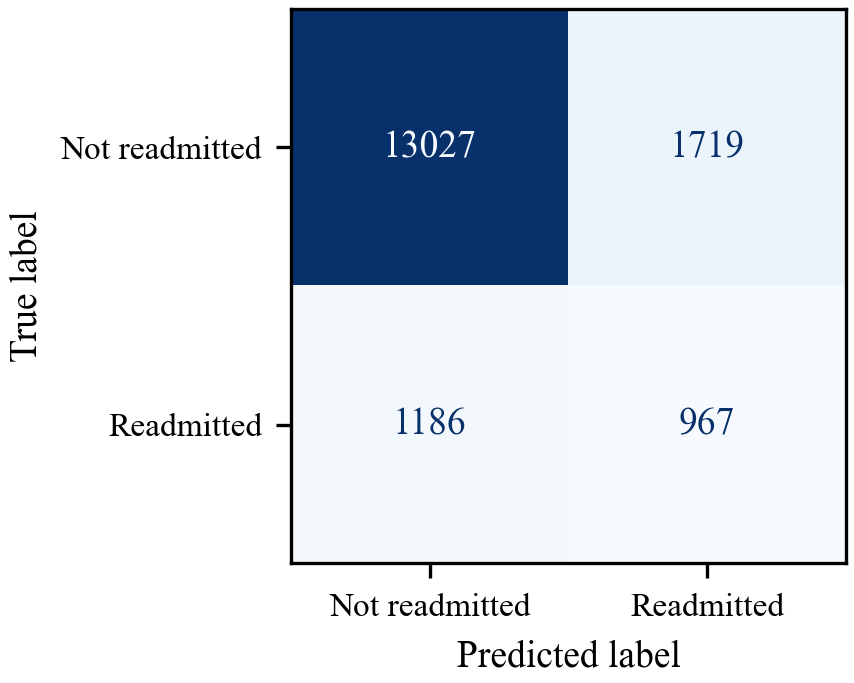
\includegraphics[width=0.78\columnwidth]{figs/fig4_confusion_matrix.png}
\caption{Confusion matrix of Logistic Regression on the test set.}
\label{fig:cm}
\end{figure}

Table~IV repeats the logistic regression pipeline under four study designs. Keeping the 7,413 in-hospital deaths raised ROC-AUC from 0.756 to 0.775 under the patient-grouped split and to 0.777 under a random split. None of these admissions was readmitted, so they are easy negatives that flatter discrimination and change the cohort prevalence. Switching from a patient-grouped to a random split changed ROC-AUC by less than 0.001 (0.756 vs 0.756), so patient overlap did not inflate results in this dataset, although the random split gave lower average precision (0.358 vs 0.372). The cohort definition is therefore a larger source of variation than the gap between any two learned models.

\begin{table}[!t]
\caption{Design Audit: Logistic Regression Under Four Study Designs}
\label{tab:audit}
\centering\footnotesize\setlength{\tabcolsep}{2.6pt}
\begin{tabular}{|l|l|r|c|c|c|c|}
\hline
\textbf{Deaths} & \textbf{Split} & \textbf{$n$ test} & \textbf{AUC} & \textbf{PR-AUC} & \textbf{Rec.} & \textbf{Prec.} \\\hline
Excluded & Grouped & 16,899 & 0.756 & 0.372 & 0.449 & 0.360 \\
Kept & Grouped & 17,981 & 0.775 & 0.375 & 0.522 & 0.324 \\
Excluded & Random & 16,889 & 0.756 & 0.358 & 0.468 & 0.319 \\
Kept & Random & 18,000 & 0.777 & 0.367 & 0.505 & 0.327 \\
\hline
\end{tabular}
\end{table}

\begin{figure*}[!t]
\centering
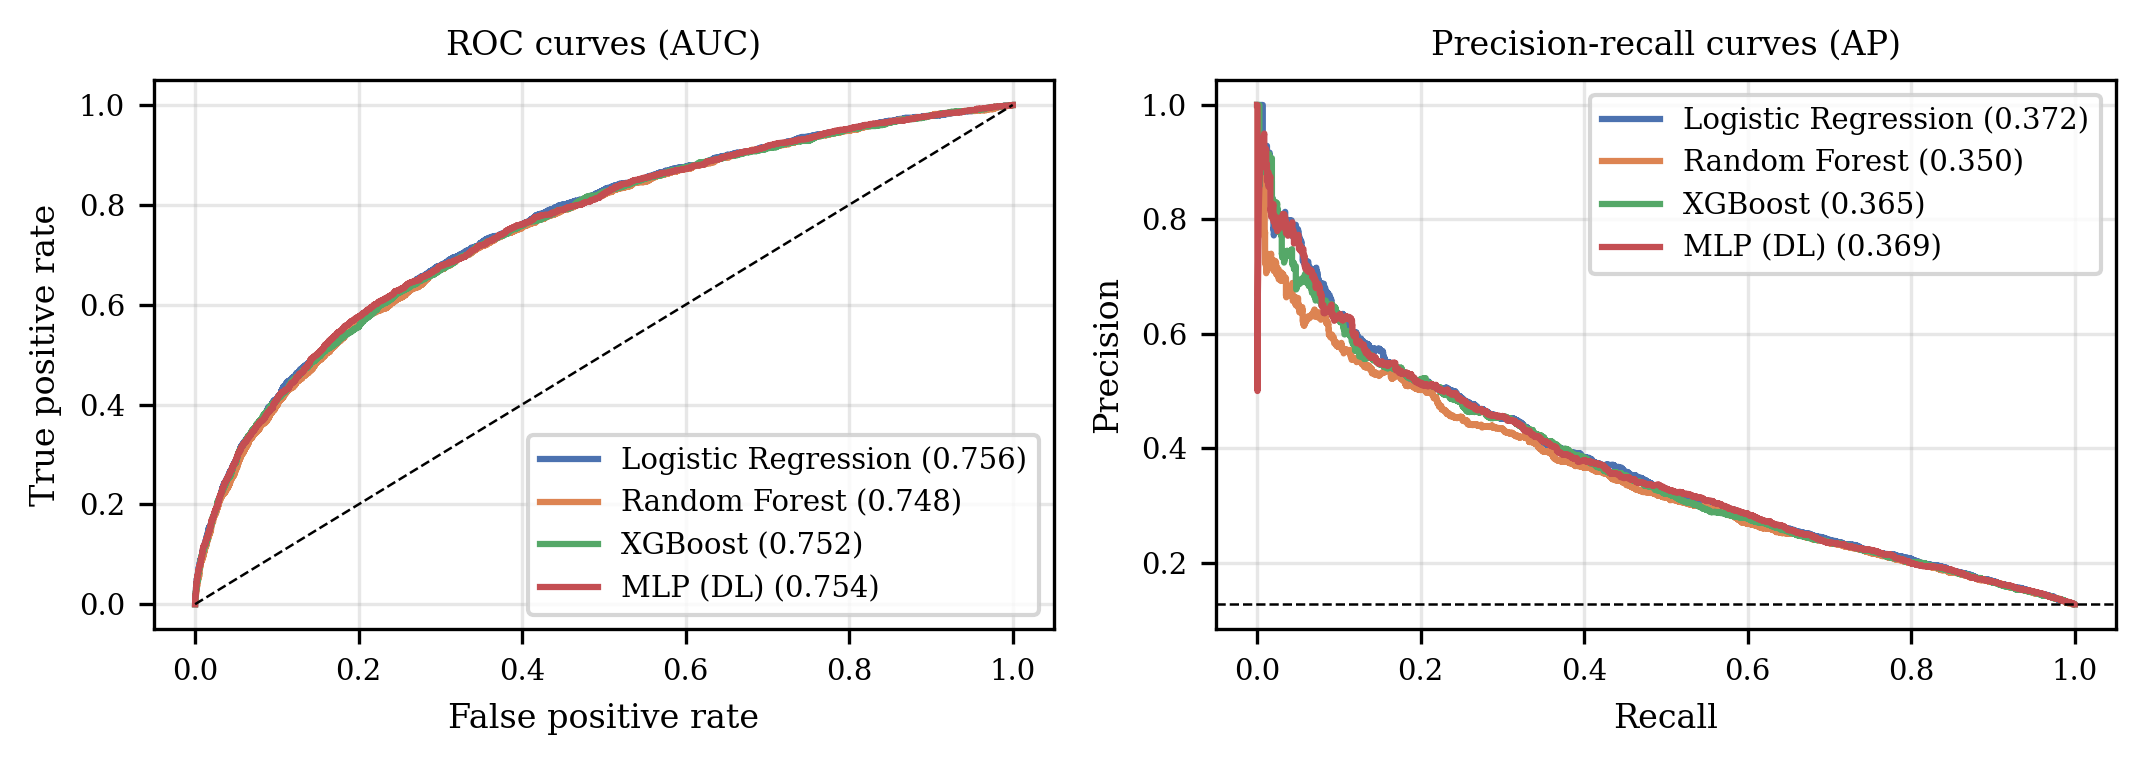
\includegraphics[width=0.8\textwidth]{figs/fig5_roc_pr.png}
\caption{ROC curves (left) and precision--recall curves (right) of the four learned models on the test set. Values in brackets are AUC and average precision.}
\label{fig:roc}
\end{figure*}

Descriptive rates agree with the model inputs. Readmission rose with age, from 6.6\% at ages 0--17 and 6.2\% at 18--39 to 19.8\% at 60--74 and 23.1\% at 75 and over. It was highest in the ICU (25.1\%), then NICU (17.7\%), HDU (14.2\%) and general wards (8.4\%), and it was higher after emergency admission (15.8\%) than after elective admission (8.8\%). It rose with the Charlson index, from 6.0\% at score 0 to 31.2\% at score 6, and it was 17.8\% after discharge against medical advice. Permutation importance ranked los days, comorbidity count, ward type and prev admissions as the four most influential inputs of the best model. The Charlson index does not appear near the top, probably because it is correlated with comorbidity count ($r{=}0.73$) and age ($r{=}0.73$). In the robustness check, the best model trained before 2024 and tested on 2024 (11,187 admissions) gave a ROC-AUC of 0.749, close to the main result. All these results describe association, not cause.

Several limits apply. The data come from one public source, and the label and sampling process were not independently verified, so external validity is untested. Inputs are limited to admission-level fields, with no medication, discharge-summary or post-discharge information. Hyperparameters were not searched, so a tuned XGBoost or MLP might narrow or reverse small gaps. Models were not recalibrated, and apart from the temporal check only one split was evaluated. The TRIPOD+AI items on external validation, calibration curves, fairness analysis and sample-size justification were not addressed, so reporting is only partly complete.

\section{Conclusion}
This work compared logistic regression, random forest, XGBoost and an MLP against a prior-only baseline for 30-day readmission, using 112,587 Indian hospital admissions, a patient-grouped split and class weighting. The learned models reached ROC-AUC values of 0.748 to 0.756 with overlapping intervals. Logistic Regression scored highest by ROC-AUC and MLP scored highest for recall, but the differences were small. Stay length, comorbidity count and ward type were the most useful inputs. The design audit showed that keeping in-hospital deaths inflated ROC-AUC by about 0.020, more than any gap between models. A simple, transparent model is a sound starting point for this kind of tabular data, and studies should state how deaths and repeat admissions were handled.

\section{Future Work}
Future work should validate the models on data from other hospitals and periods, verify how the dataset labels were generated, and tune hyperparameters with cross-validation. Recalibration and threshold analysis for specific follow-up programmes are also needed. Adding discharge summaries, medications and post-discharge data may raise performance beyond the present level, and explainability methods such as SHAP could support clinical use.

\bibliographystyle{IEEEtran}
\bibliography{refs}
\end{document}
